% Options for packages loaded elsewhere
\PassOptionsToPackage{unicode}{hyperref}
\PassOptionsToPackage{hyphens}{url}
\PassOptionsToPackage{dvipsnames,svgnames,x11names}{xcolor}
%
\documentclass[
  letterpaper,
  DIV=11,
  numbers=noendperiod]{scrartcl}

\usepackage{amsmath,amssymb}
\usepackage{iftex}
\ifPDFTeX
  \usepackage[T1]{fontenc}
  \usepackage[utf8]{inputenc}
  \usepackage{textcomp} % provide euro and other symbols
\else % if luatex or xetex
  \usepackage{unicode-math}
  \defaultfontfeatures{Scale=MatchLowercase}
  \defaultfontfeatures[\rmfamily]{Ligatures=TeX,Scale=1}
\fi
\usepackage{lmodern}
\ifPDFTeX\else  
    % xetex/luatex font selection
\fi
% Use upquote if available, for straight quotes in verbatim environments
\IfFileExists{upquote.sty}{\usepackage{upquote}}{}
\IfFileExists{microtype.sty}{% use microtype if available
  \usepackage[]{microtype}
  \UseMicrotypeSet[protrusion]{basicmath} % disable protrusion for tt fonts
}{}
\makeatletter
\@ifundefined{KOMAClassName}{% if non-KOMA class
  \IfFileExists{parskip.sty}{%
    \usepackage{parskip}
  }{% else
    \setlength{\parindent}{0pt}
    \setlength{\parskip}{6pt plus 2pt minus 1pt}}
}{% if KOMA class
  \KOMAoptions{parskip=half}}
\makeatother
\usepackage{xcolor}
\setlength{\emergencystretch}{3em} % prevent overfull lines
\setcounter{secnumdepth}{-\maxdimen} % remove section numbering
% Make \paragraph and \subparagraph free-standing
\makeatletter
\ifx\paragraph\undefined\else
  \let\oldparagraph\paragraph
  \renewcommand{\paragraph}{
    \@ifstar
      \xxxParagraphStar
      \xxxParagraphNoStar
  }
  \newcommand{\xxxParagraphStar}[1]{\oldparagraph*{#1}\mbox{}}
  \newcommand{\xxxParagraphNoStar}[1]{\oldparagraph{#1}\mbox{}}
\fi
\ifx\subparagraph\undefined\else
  \let\oldsubparagraph\subparagraph
  \renewcommand{\subparagraph}{
    \@ifstar
      \xxxSubParagraphStar
      \xxxSubParagraphNoStar
  }
  \newcommand{\xxxSubParagraphStar}[1]{\oldsubparagraph*{#1}\mbox{}}
  \newcommand{\xxxSubParagraphNoStar}[1]{\oldsubparagraph{#1}\mbox{}}
\fi
\makeatother

\usepackage{color}
\usepackage{fancyvrb}
\newcommand{\VerbBar}{|}
\newcommand{\VERB}{\Verb[commandchars=\\\{\}]}
\DefineVerbatimEnvironment{Highlighting}{Verbatim}{commandchars=\\\{\}}
% Add ',fontsize=\small' for more characters per line
\usepackage{framed}
\definecolor{shadecolor}{RGB}{241,243,245}
\newenvironment{Shaded}{\begin{snugshade}}{\end{snugshade}}
\newcommand{\AlertTok}[1]{\textcolor[rgb]{0.68,0.00,0.00}{#1}}
\newcommand{\AnnotationTok}[1]{\textcolor[rgb]{0.37,0.37,0.37}{#1}}
\newcommand{\AttributeTok}[1]{\textcolor[rgb]{0.40,0.45,0.13}{#1}}
\newcommand{\BaseNTok}[1]{\textcolor[rgb]{0.68,0.00,0.00}{#1}}
\newcommand{\BuiltInTok}[1]{\textcolor[rgb]{0.00,0.23,0.31}{#1}}
\newcommand{\CharTok}[1]{\textcolor[rgb]{0.13,0.47,0.30}{#1}}
\newcommand{\CommentTok}[1]{\textcolor[rgb]{0.37,0.37,0.37}{#1}}
\newcommand{\CommentVarTok}[1]{\textcolor[rgb]{0.37,0.37,0.37}{\textit{#1}}}
\newcommand{\ConstantTok}[1]{\textcolor[rgb]{0.56,0.35,0.01}{#1}}
\newcommand{\ControlFlowTok}[1]{\textcolor[rgb]{0.00,0.23,0.31}{\textbf{#1}}}
\newcommand{\DataTypeTok}[1]{\textcolor[rgb]{0.68,0.00,0.00}{#1}}
\newcommand{\DecValTok}[1]{\textcolor[rgb]{0.68,0.00,0.00}{#1}}
\newcommand{\DocumentationTok}[1]{\textcolor[rgb]{0.37,0.37,0.37}{\textit{#1}}}
\newcommand{\ErrorTok}[1]{\textcolor[rgb]{0.68,0.00,0.00}{#1}}
\newcommand{\ExtensionTok}[1]{\textcolor[rgb]{0.00,0.23,0.31}{#1}}
\newcommand{\FloatTok}[1]{\textcolor[rgb]{0.68,0.00,0.00}{#1}}
\newcommand{\FunctionTok}[1]{\textcolor[rgb]{0.28,0.35,0.67}{#1}}
\newcommand{\ImportTok}[1]{\textcolor[rgb]{0.00,0.46,0.62}{#1}}
\newcommand{\InformationTok}[1]{\textcolor[rgb]{0.37,0.37,0.37}{#1}}
\newcommand{\KeywordTok}[1]{\textcolor[rgb]{0.00,0.23,0.31}{\textbf{#1}}}
\newcommand{\NormalTok}[1]{\textcolor[rgb]{0.00,0.23,0.31}{#1}}
\newcommand{\OperatorTok}[1]{\textcolor[rgb]{0.37,0.37,0.37}{#1}}
\newcommand{\OtherTok}[1]{\textcolor[rgb]{0.00,0.23,0.31}{#1}}
\newcommand{\PreprocessorTok}[1]{\textcolor[rgb]{0.68,0.00,0.00}{#1}}
\newcommand{\RegionMarkerTok}[1]{\textcolor[rgb]{0.00,0.23,0.31}{#1}}
\newcommand{\SpecialCharTok}[1]{\textcolor[rgb]{0.37,0.37,0.37}{#1}}
\newcommand{\SpecialStringTok}[1]{\textcolor[rgb]{0.13,0.47,0.30}{#1}}
\newcommand{\StringTok}[1]{\textcolor[rgb]{0.13,0.47,0.30}{#1}}
\newcommand{\VariableTok}[1]{\textcolor[rgb]{0.07,0.07,0.07}{#1}}
\newcommand{\VerbatimStringTok}[1]{\textcolor[rgb]{0.13,0.47,0.30}{#1}}
\newcommand{\WarningTok}[1]{\textcolor[rgb]{0.37,0.37,0.37}{\textit{#1}}}

\providecommand{\tightlist}{%
  \setlength{\itemsep}{0pt}\setlength{\parskip}{0pt}}\usepackage{longtable,booktabs,array}
\usepackage{calc} % for calculating minipage widths
% Correct order of tables after \paragraph or \subparagraph
\usepackage{etoolbox}
\makeatletter
\patchcmd\longtable{\par}{\if@noskipsec\mbox{}\fi\par}{}{}
\makeatother
% Allow footnotes in longtable head/foot
\IfFileExists{footnotehyper.sty}{\usepackage{footnotehyper}}{\usepackage{footnote}}
\makesavenoteenv{longtable}
\usepackage{graphicx}
\makeatletter
\def\maxwidth{\ifdim\Gin@nat@width>\linewidth\linewidth\else\Gin@nat@width\fi}
\def\maxheight{\ifdim\Gin@nat@height>\textheight\textheight\else\Gin@nat@height\fi}
\makeatother
% Scale images if necessary, so that they will not overflow the page
% margins by default, and it is still possible to overwrite the defaults
% using explicit options in \includegraphics[width, height, ...]{}
\setkeys{Gin}{width=\maxwidth,height=\maxheight,keepaspectratio}
% Set default figure placement to htbp
\makeatletter
\def\fps@figure{htbp}
\makeatother

\KOMAoption{captions}{tableheading}
\makeatletter
\@ifpackageloaded{caption}{}{\usepackage{caption}}
\AtBeginDocument{%
\ifdefined\contentsname
  \renewcommand*\contentsname{Table of contents}
\else
  \newcommand\contentsname{Table of contents}
\fi
\ifdefined\listfigurename
  \renewcommand*\listfigurename{List of Figures}
\else
  \newcommand\listfigurename{List of Figures}
\fi
\ifdefined\listtablename
  \renewcommand*\listtablename{List of Tables}
\else
  \newcommand\listtablename{List of Tables}
\fi
\ifdefined\figurename
  \renewcommand*\figurename{Figure}
\else
  \newcommand\figurename{Figure}
\fi
\ifdefined\tablename
  \renewcommand*\tablename{Table}
\else
  \newcommand\tablename{Table}
\fi
}
\@ifpackageloaded{float}{}{\usepackage{float}}
\floatstyle{ruled}
\@ifundefined{c@chapter}{\newfloat{codelisting}{h}{lop}}{\newfloat{codelisting}{h}{lop}[chapter]}
\floatname{codelisting}{Listing}
\newcommand*\listoflistings{\listof{codelisting}{List of Listings}}
\makeatother
\makeatletter
\makeatother
\makeatletter
\@ifpackageloaded{caption}{}{\usepackage{caption}}
\@ifpackageloaded{subcaption}{}{\usepackage{subcaption}}
\makeatother

\ifLuaTeX
  \usepackage{selnolig}  % disable illegal ligatures
\fi
\usepackage{bookmark}

\IfFileExists{xurl.sty}{\usepackage{xurl}}{} % add URL line breaks if available
\urlstyle{same} % disable monospaced font for URLs
\hypersetup{
  pdftitle={Class 9: Structural Bioinformatics (pt.1)},
  pdfauthor={Sofia Lanaspa, A17105313},
  colorlinks=true,
  linkcolor={blue},
  filecolor={Maroon},
  citecolor={Blue},
  urlcolor={Blue},
  pdfcreator={LaTeX via pandoc}}


\title{Class 9: Structural Bioinformatics (pt.1)}
\author{Sofia Lanaspa, A17105313}
\date{}

\begin{document}
\maketitle


The main database for strucutal data on proteins is PDB(protein data
book), let see what it contain:

Data from: https://www.rcsb.org/stats

\begin{Shaded}
\begin{Highlighting}[]
\NormalTok{pdbdb }\OtherTok{\textless{}{-}} \FunctionTok{read.csv}\NormalTok{(}\StringTok{"Data Export Summary.csv"}\NormalTok{)}
\end{Highlighting}
\end{Shaded}

\begin{Shaded}
\begin{Highlighting}[]
\NormalTok{pdbdb}\SpecialCharTok{$}\NormalTok{total}
\end{Highlighting}
\end{Shaded}

\begin{verbatim}
NULL
\end{verbatim}

\begin{Shaded}
\begin{Highlighting}[]
\CommentTok{\#issue because numbers are in quotes due to the coma}
\FunctionTok{as.numeric}\NormalTok{(}\FunctionTok{sub}\NormalTok{(}\StringTok{","}\NormalTok{,}\StringTok{""}\NormalTok{,pdbdb}\SpecialCharTok{$}\NormalTok{Total)) }\CommentTok{\#convert values to numeric to do math}
\end{Highlighting}
\end{Shaded}

\begin{verbatim}
[1] 195610  12318  13720   4531    213     22
\end{verbatim}

Could turn the code above into a function

\begin{Shaded}
\begin{Highlighting}[]
\NormalTok{comma2numeric }\OtherTok{\textless{}{-}} \ControlFlowTok{function}\NormalTok{(x)\{}
  \FunctionTok{as.numeric}\NormalTok{(}\FunctionTok{sub}\NormalTok{(}\StringTok{","}\NormalTok{,}\StringTok{""}\NormalTok{,x))}
\NormalTok{\}}
\FunctionTok{comma2numeric}\NormalTok{((pdbdb}\SpecialCharTok{$}\NormalTok{X.ray)) }\CommentTok{\#test function}
\end{Highlighting}
\end{Shaded}

\begin{verbatim}
[1] 167192   9639   8730   2869    170     11
\end{verbatim}

\begin{Shaded}
\begin{Highlighting}[]
\FunctionTok{apply}\NormalTok{(pdbdb,}\DecValTok{2}\NormalTok{,comma2numeric)}
\end{Highlighting}
\end{Shaded}

\begin{verbatim}
Warning in FUN(newX[, i], ...): NAs introduced by coercion
\end{verbatim}

\begin{verbatim}
     Molecular.Type  X.ray    EM   NMR Multiple.methods Neutron Other  Total
[1,]             NA 167192 15572 12529              208      77    32 195610
[2,]             NA   9639  2635    34                8       2     0  12318
[3,]             NA   8730  4697   286                7       0     0  13720
[4,]             NA   2869   137  1507               14       3     1   4531
[5,]             NA    170    10    33                0       0     0    213
[6,]             NA     11     0     6                1       0     4     22
\end{verbatim}

OR TRY DIFFERENT FUNCTION

\begin{Shaded}
\begin{Highlighting}[]
\FunctionTok{library}\NormalTok{(readr)}
\NormalTok{pdbdb }\OtherTok{\textless{}{-}} \FunctionTok{read\_csv}\NormalTok{(}\StringTok{"Data Export Summary.csv"}\NormalTok{)}
\end{Highlighting}
\end{Shaded}

\begin{verbatim}
Rows: 6 Columns: 8
-- Column specification --------------------------------------------------------
Delimiter: ","
chr (1): Molecular Type
dbl (3): Multiple methods, Neutron, Other
num (4): X-ray, EM, NMR, Total

i Use `spec()` to retrieve the full column specification for this data.
i Specify the column types or set `show_col_types = FALSE` to quiet this message.
\end{verbatim}

\paragraph{Q1: What percentage of structures in the PDB are solved by
X-Ray and Electron
Microscopy}\label{q1-what-percentage-of-structures-in-the-pdb-are-solved-by-x-ray-and-electron-microscopy}

\begin{Shaded}
\begin{Highlighting}[]
\CommentTok{\#Sum of all x{-}rays divided the Total}
\NormalTok{(}\FunctionTok{sum}\NormalTok{(pdbdb}\SpecialCharTok{$}\StringTok{"X{-}ray"}\NormalTok{)}\SpecialCharTok{/}\FunctionTok{sum}\NormalTok{(pdbdb}\SpecialCharTok{$}\NormalTok{Total)) }\SpecialCharTok{*} \DecValTok{100}
\end{Highlighting}
\end{Shaded}

\begin{verbatim}
[1] 83.30359
\end{verbatim}

\paragraph{Q2: What proportion of structures in the PDB are
protein?}\label{q2-what-proportion-of-structures-in-the-pdb-are-protein}

\begin{Shaded}
\begin{Highlighting}[]
\CommentTok{\#First value of column \textquotesingle{}Total\textquotesingle{} is only protein, divided by all the values in \textquotesingle{}Total\textquotesingle{}}
\NormalTok{(pdbdb}\SpecialCharTok{$}\NormalTok{Total[}\DecValTok{1}\NormalTok{]}\SpecialCharTok{/} \FunctionTok{sum}\NormalTok{(pdbdb}\SpecialCharTok{$}\NormalTok{Total)) }\SpecialCharTok{*} \DecValTok{100}
\end{Highlighting}
\end{Shaded}

\begin{verbatim}
[1] 86.39483
\end{verbatim}

\paragraph{Q3: Type HIV in the PDB website search box on the home page
and determine how many HIV-1 protease structures are in the current
PDB?}\label{q3-type-hiv-in-the-pdb-website-search-box-on-the-home-page-and-determine-how-many-hiv-1-protease-structures-are-in-the-current-pdb}

\begin{Shaded}
\begin{Highlighting}[]
\CommentTok{\#Look up HIV on website, number of results = 4,553}
\end{Highlighting}
\end{Shaded}

\paragraph{Q4: Water molecules normally have 3 atoms. Why do we see just
one atom per water molecule in this
structure?}\label{q4-water-molecules-normally-have-3-atoms.-why-do-we-see-just-one-atom-per-water-molecule-in-this-structure}

\begin{Shaded}
\begin{Highlighting}[]
\CommentTok{\# because the diagram focuses on the central oxygen atom}
\end{Highlighting}
\end{Shaded}

\paragraph{Q6: Generate and save a figure clearly showing the two
distinct chains of HIV-protease along with the ligand. You might also
consider showing the catalytic residues ASP 25 in each chain and the
critical water (we recommend ``Ball \& Stick'' for these side-chains).
Add this figure to your Quarto
document.}\label{q6-generate-and-save-a-figure-clearly-showing-the-two-distinct-chains-of-hiv-protease-along-with-the-ligand.-you-might-also-consider-showing-the-catalytic-residues-asp-25-in-each-chain-and-the-critical-water-we-recommend-ball-stick-for-these-side-chains.-add-this-figure-to-your-quarto-document.}

\paragraph{Discussion Topic: Can you think of a way in which indinavir,
or even larger ligands and substrates, could enter the binding
site?}\label{discussion-topic-can-you-think-of-a-way-in-which-indinavir-or-even-larger-ligands-and-substrates-could-enter-the-binding-site}

\paragraph{Q7: {[}Optional{]} As you have hopefully observed HIV
protease is a homodimer (i.e.~it is composed of two identical chains).
With the aid of the graphic display can you identify secondary structure
elements that are likely to only form in the dimer rather than the
monomer?}\label{q7-optional-as-you-have-hopefully-observed-hiv-protease-is-a-homodimer-i.e.-it-is-composed-of-two-identical-chains.-with-the-aid-of-the-graphic-display-can-you-identify-secondary-structure-elements-that-are-likely-to-only-form-in-the-dimer-rather-than-the-monomer}

Import image from molstar (https://molstar.org/viewer/):
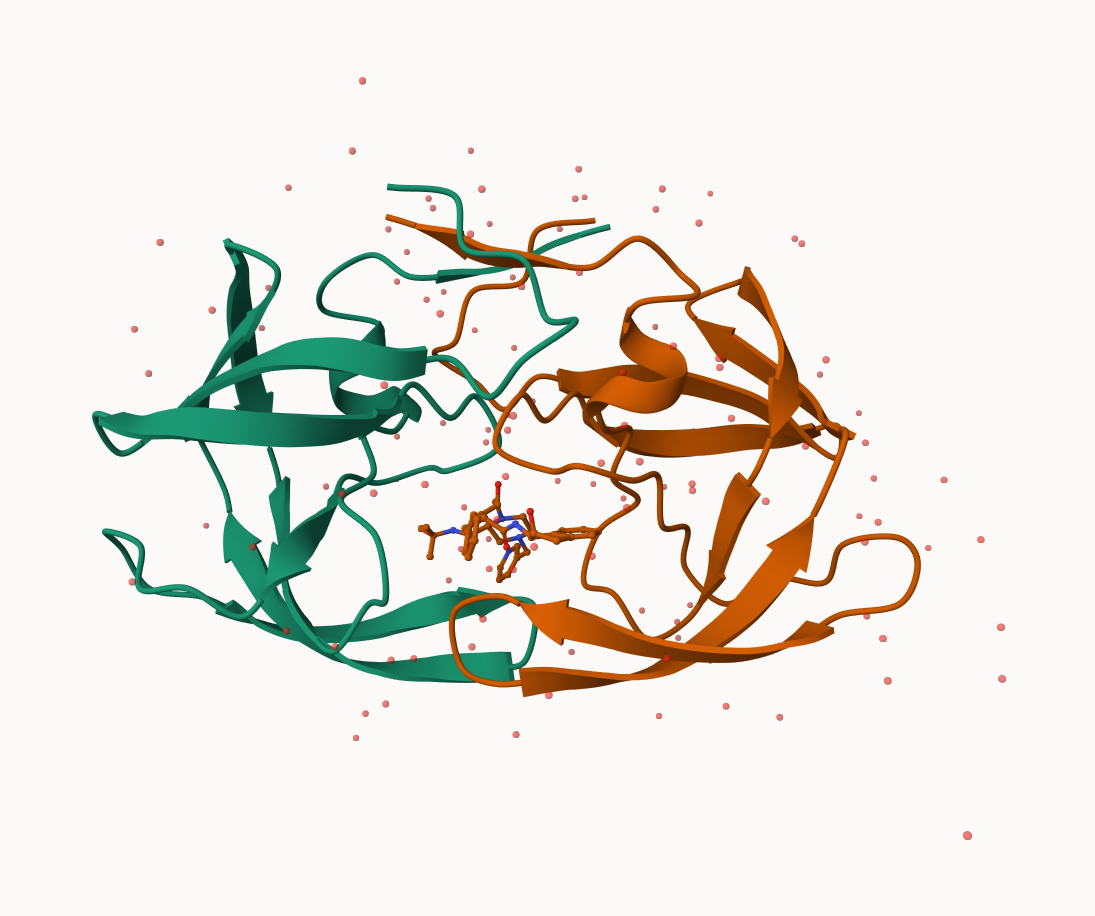
\includegraphics{1HSG.png}

Steps to edit this protein structure:

click arrow on right side - select D25 (aspartate) - 3D box - set
representation to `spacefill' - do the same for chain B to visualize it
in a more realistic way, and see where the ligand binds: on right hand
side click components - add - selection = `polymer' - representation =
`molecular surface' - add component 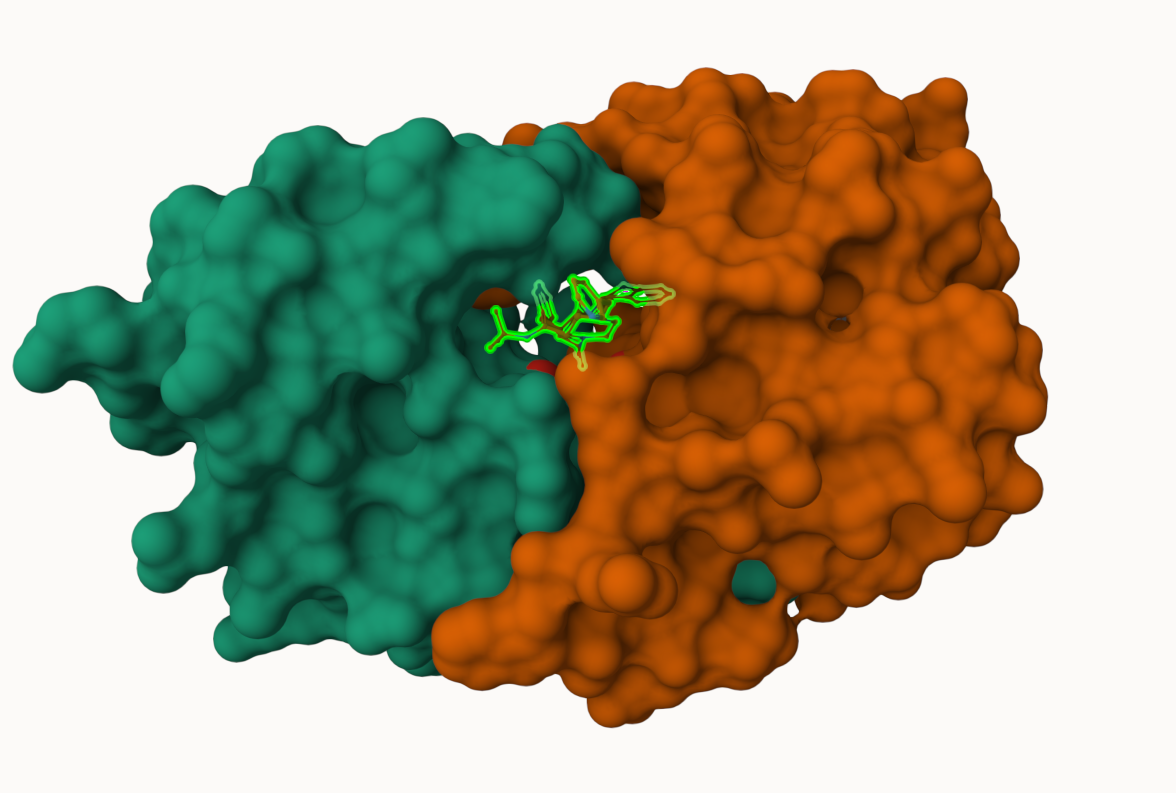
\includegraphics{1HSG-2.png}

\subsection{Bio3D}\label{bio3d}

The Bio3D pachage allows us to do all sorts of structural bioinformatics
work in R.

Let's start with how it can read PDB files:

\begin{Shaded}
\begin{Highlighting}[]
\FunctionTok{library}\NormalTok{(bio3d)}
\NormalTok{pdb }\OtherTok{\textless{}{-}} \FunctionTok{read.pdb}\NormalTok{(}\StringTok{"1hsg"}\NormalTok{)}
\end{Highlighting}
\end{Shaded}

\begin{verbatim}
  Note: Accessing on-line PDB file
\end{verbatim}

\begin{Shaded}
\begin{Highlighting}[]
\NormalTok{pdb}
\end{Highlighting}
\end{Shaded}

\begin{verbatim}

 Call:  read.pdb(file = "1hsg")

   Total Models#: 1
     Total Atoms#: 1686,  XYZs#: 5058  Chains#: 2  (values: A B)

     Protein Atoms#: 1514  (residues/Calpha atoms#: 198)
     Nucleic acid Atoms#: 0  (residues/phosphate atoms#: 0)

     Non-protein/nucleic Atoms#: 172  (residues: 128)
     Non-protein/nucleic resid values: [ HOH (127), MK1 (1) ]

   Protein sequence:
      PQITLWQRPLVTIKIGGQLKEALLDTGADDTVLEEMSLPGRWKPKMIGGIGGFIKVRQYD
      QILIEICGHKAIGTVLVGPTPVNIIGRNLLTQIGCTLNFPQITLWQRPLVTIKIGGQLKE
      ALLDTGADDTVLEEMSLPGRWKPKMIGGIGGFIKVRQYDQILIEICGHKAIGTVLVGPTP
      VNIIGRNLLTQIGCTLNF

+ attr: atom, xyz, seqres, helix, sheet,
        calpha, remark, call
\end{verbatim}

\begin{Shaded}
\begin{Highlighting}[]
\FunctionTok{attributes}\NormalTok{(pdb)}
\end{Highlighting}
\end{Shaded}

\begin{verbatim}
$names
[1] "atom"   "xyz"    "seqres" "helix"  "sheet"  "calpha" "remark" "call"  

$class
[1] "pdb" "sse"
\end{verbatim}

\begin{Shaded}
\begin{Highlighting}[]
\FunctionTok{head}\NormalTok{(pdb}\SpecialCharTok{$}\NormalTok{atom)}
\end{Highlighting}
\end{Shaded}

\begin{verbatim}
  type eleno elety  alt resid chain resno insert      x      y     z o     b
1 ATOM     1     N <NA>   PRO     A     1   <NA> 29.361 39.686 5.862 1 38.10
2 ATOM     2    CA <NA>   PRO     A     1   <NA> 30.307 38.663 5.319 1 40.62
3 ATOM     3     C <NA>   PRO     A     1   <NA> 29.760 38.071 4.022 1 42.64
4 ATOM     4     O <NA>   PRO     A     1   <NA> 28.600 38.302 3.676 1 43.40
5 ATOM     5    CB <NA>   PRO     A     1   <NA> 30.508 37.541 6.342 1 37.87
6 ATOM     6    CG <NA>   PRO     A     1   <NA> 29.296 37.591 7.162 1 38.40
  segid elesy charge
1  <NA>     N   <NA>
2  <NA>     C   <NA>
3  <NA>     C   <NA>
4  <NA>     O   <NA>
5  <NA>     C   <NA>
6  <NA>     C   <NA>
\end{verbatim}

\begin{Shaded}
\begin{Highlighting}[]
\FunctionTok{pdbseq}\NormalTok{(pdb)}
\end{Highlighting}
\end{Shaded}

\begin{verbatim}
  1   2   3   4   5   6   7   8   9  10  11  12  13  14  15  16  17  18  19  20 
"P" "Q" "I" "T" "L" "W" "Q" "R" "P" "L" "V" "T" "I" "K" "I" "G" "G" "Q" "L" "K" 
 21  22  23  24  25  26  27  28  29  30  31  32  33  34  35  36  37  38  39  40 
"E" "A" "L" "L" "D" "T" "G" "A" "D" "D" "T" "V" "L" "E" "E" "M" "S" "L" "P" "G" 
 41  42  43  44  45  46  47  48  49  50  51  52  53  54  55  56  57  58  59  60 
"R" "W" "K" "P" "K" "M" "I" "G" "G" "I" "G" "G" "F" "I" "K" "V" "R" "Q" "Y" "D" 
 61  62  63  64  65  66  67  68  69  70  71  72  73  74  75  76  77  78  79  80 
"Q" "I" "L" "I" "E" "I" "C" "G" "H" "K" "A" "I" "G" "T" "V" "L" "V" "G" "P" "T" 
 81  82  83  84  85  86  87  88  89  90  91  92  93  94  95  96  97  98  99   1 
"P" "V" "N" "I" "I" "G" "R" "N" "L" "L" "T" "Q" "I" "G" "C" "T" "L" "N" "F" "P" 
  2   3   4   5   6   7   8   9  10  11  12  13  14  15  16  17  18  19  20  21 
"Q" "I" "T" "L" "W" "Q" "R" "P" "L" "V" "T" "I" "K" "I" "G" "G" "Q" "L" "K" "E" 
 22  23  24  25  26  27  28  29  30  31  32  33  34  35  36  37  38  39  40  41 
"A" "L" "L" "D" "T" "G" "A" "D" "D" "T" "V" "L" "E" "E" "M" "S" "L" "P" "G" "R" 
 42  43  44  45  46  47  48  49  50  51  52  53  54  55  56  57  58  59  60  61 
"W" "K" "P" "K" "M" "I" "G" "G" "I" "G" "G" "F" "I" "K" "V" "R" "Q" "Y" "D" "Q" 
 62  63  64  65  66  67  68  69  70  71  72  73  74  75  76  77  78  79  80  81 
"I" "L" "I" "E" "I" "C" "G" "H" "K" "A" "I" "G" "T" "V" "L" "V" "G" "P" "T" "P" 
 82  83  84  85  86  87  88  89  90  91  92  93  94  95  96  97  98  99 
"V" "N" "I" "I" "G" "R" "N" "L" "L" "T" "Q" "I" "G" "C" "T" "L" "N" "F" 
\end{verbatim}

\begin{Shaded}
\begin{Highlighting}[]
\FunctionTok{pdbseq}\NormalTok{(pdb)[}\DecValTok{25}\NormalTok{] }\CommentTok{\#number gives you amino acid at that position }
\end{Highlighting}
\end{Shaded}

\begin{verbatim}
 25 
"D" 
\end{verbatim}

\paragraph{Q7: How many amino acid residues are there in this pdb
object?}\label{q7-how-many-amino-acid-residues-are-there-in-this-pdb-object}

\begin{Shaded}
\begin{Highlighting}[]
\FunctionTok{sum}\NormalTok{(pdb}\SpecialCharTok{$}\NormalTok{calpha) }\CommentTok{\#there is 1 calpha per AA so count calpha\textquotesingle{}s}
\end{Highlighting}
\end{Shaded}

\begin{verbatim}
[1] 198
\end{verbatim}

\begin{Shaded}
\begin{Highlighting}[]
\FunctionTok{length}\NormalTok{(pdb)}
\end{Highlighting}
\end{Shaded}

\begin{verbatim}
[1] 8
\end{verbatim}

\paragraph{Q8: Name one of the two non-protein
residues?}\label{q8-name-one-of-the-two-non-protein-residues}

\begin{Shaded}
\begin{Highlighting}[]
\CommentTok{\#HOH, MK1}
\end{Highlighting}
\end{Shaded}

\paragraph{Q9: How many protein chains are in this
structure?}\label{q9-how-many-protein-chains-are-in-this-structure}

\begin{Shaded}
\begin{Highlighting}[]
\CommentTok{\# 2 chains}
\end{Highlighting}
\end{Shaded}

\begin{Shaded}
\begin{Highlighting}[]
\NormalTok{adk }\OtherTok{\textless{}{-}} \FunctionTok{read.pdb}\NormalTok{(}\StringTok{"3s36"}\NormalTok{)}
\end{Highlighting}
\end{Shaded}

\begin{verbatim}
  Note: Accessing on-line PDB file
\end{verbatim}

\begin{Shaded}
\begin{Highlighting}[]
\NormalTok{adk}
\end{Highlighting}
\end{Shaded}

\begin{verbatim}

 Call:  read.pdb(file = "3s36")

   Total Models#: 1
     Total Atoms#: 4104,  XYZs#: 12312  Chains#: 3  (values: L H X)

     Protein Atoms#: 4104  (residues/Calpha atoms#: 540)
     Nucleic acid Atoms#: 0  (residues/phosphate atoms#: 0)

     Non-protein/nucleic Atoms#: 0  (residues: 0)
     Non-protein/nucleic resid values: [ none ]

   Protein sequence:
      DIQMTQSPSSVSASIGDRVTITCRASQGIDNWLGWYQQKPGKAPKLLIYDASNLDTGVPS
      RFSGSGSGTYFTLTISSLQAEDFAVYFCQQAKAFPPTFGGGTKVDIKRTVAAPSVFIFPP
      SDEQLKSGTASVVCLLNNFYPREAKVQWKVDNALQSGNSQESVTEQDSKDSTYSLSSTLT
      LSKADYEKHKVYACEVTHQGLSSPVTKSFNRGECVQLVQSGGGLV...<cut>...KPFV

+ attr: atom, xyz, seqres, helix, sheet,
        calpha, remark, call
\end{verbatim}

\begin{Shaded}
\begin{Highlighting}[]
\CommentTok{\# Perform fleibility prediction }
\NormalTok{m }\OtherTok{\textless{}{-}} \FunctionTok{nma}\NormalTok{(adk)}
\end{Highlighting}
\end{Shaded}

\begin{verbatim}
Warning in nma.pdb(adk): Possible multi-chain structure or missing in-structure residue(s) present
  Fluctuations at neighboring positions may be affected.
\end{verbatim}

\begin{verbatim}
 Building Hessian...        Done in 0.059 seconds.
 Diagonalizing Hessian...   Done in 3.577 seconds.
\end{verbatim}

\begin{Shaded}
\begin{Highlighting}[]
\FunctionTok{plot}\NormalTok{(m)}
\end{Highlighting}
\end{Shaded}

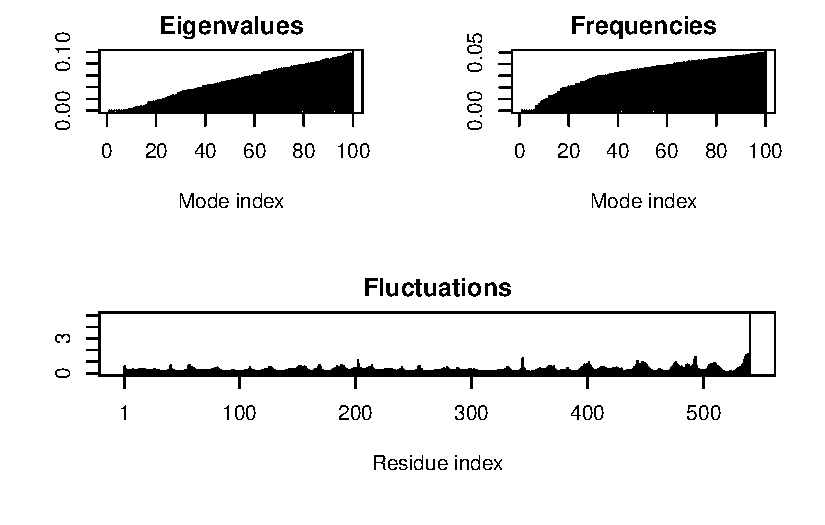
\includegraphics{BIMM143-Lab-9-final_files/figure-pdf/unnamed-chunk-18-1.pdf}

Write out multi-model PDB file (trajectory) that we can use to make an
animation or the predicted motions

\begin{Shaded}
\begin{Highlighting}[]
\FunctionTok{mktrj}\NormalTok{(m, }\AttributeTok{file=}\StringTok{"adk.pdb"}\NormalTok{)}
\end{Highlighting}
\end{Shaded}

I can open this in Mol* to play the trajectory\ldots{}

\subsection{Comparative analysis of Protein
Structure}\label{comparative-analysis-of-protein-structure}

\begin{Shaded}
\begin{Highlighting}[]
\FunctionTok{library}\NormalTok{(bio3d)}
\end{Highlighting}
\end{Shaded}

Here we will find and analyze all ADK structures in the PDB database

We will start with a single database accession id: ``1ake\_A''

\begin{Shaded}
\begin{Highlighting}[]
\NormalTok{id }\OtherTok{\textless{}{-}} \StringTok{"1ake\_A"}
\NormalTok{aa }\OtherTok{\textless{}{-}} \FunctionTok{get.seq}\NormalTok{(id)}
\end{Highlighting}
\end{Shaded}

\begin{verbatim}
Warning in get.seq(id): Removing existing file: seqs.fasta
\end{verbatim}

\begin{verbatim}
Fetching... Please wait. Done.
\end{verbatim}

\paragraph{Question 10}\label{question-10}

Q10. Which of the packages above is found only on BioConductor and not
CRAN?

\begin{Shaded}
\begin{Highlighting}[]
\CommentTok{\# BioConductor is a different set of packges only for biology tools, the \textquotesingle{}msa\textquotesingle{} package is from BioConductor}
\end{Highlighting}
\end{Shaded}

I ran these cmds int the R console:

install.packages(``BiocManager'') BiocManager::install(``msa'')

\paragraph{Question 13}\label{question-13}

Q13. How many amino acids are in this sequence, i.e.~how long is this
sequence?

\begin{Shaded}
\begin{Highlighting}[]
\FunctionTok{length}\NormalTok{(aa}\SpecialCharTok{$}\NormalTok{ali)}
\end{Highlighting}
\end{Shaded}

\begin{verbatim}
[1] 214
\end{verbatim}

\begin{Shaded}
\begin{Highlighting}[]
\NormalTok{aa}\SpecialCharTok{$}\NormalTok{call}
\end{Highlighting}
\end{Shaded}

\begin{verbatim}
read.fasta(file = outfile)
\end{verbatim}

\begin{Shaded}
\begin{Highlighting}[]
\NormalTok{b }\OtherTok{\textless{}{-}} \FunctionTok{blast.pdb}\NormalTok{(aa)}
\end{Highlighting}
\end{Shaded}

\begin{verbatim}
 Searching ... please wait (updates every 5 seconds) RID = JMW7XN7Z016 
 ...
 Reporting 85 hits
\end{verbatim}

\begin{Shaded}
\begin{Highlighting}[]
\CommentTok{\# fun fact: government website on election day so might block user}
\end{Highlighting}
\end{Shaded}

\begin{Shaded}
\begin{Highlighting}[]
\FunctionTok{head}\NormalTok{(b)}
\end{Highlighting}
\end{Shaded}

\begin{verbatim}
$hit.tbl
         queryid subjectids identity alignmentlength mismatches gapopens
1  Query_3847869     1AKE_A  100.000             214          0        0
2  Query_3847869     8BQF_A   99.533             214          1        0
3  Query_3847869     4X8M_A   99.533             214          1        0
4  Query_3847869     6S36_A   99.533             214          1        0
5  Query_3847869     8Q2B_A   99.533             214          1        0
6  Query_3847869     8RJ9_A   99.533             214          1        0
7  Query_3847869     6RZE_A   99.533             214          1        0
8  Query_3847869     4X8H_A   99.533             214          1        0
9  Query_3847869     3HPR_A   99.533             214          1        0
10 Query_3847869     1E4V_A   99.533             214          1        0
11 Query_3847869     5EJE_A   99.065             214          2        0
12 Query_3847869     1E4Y_A   99.065             214          2        0
13 Query_3847869     3X2S_A   98.598             214          3        0
14 Query_3847869     6HAP_A   98.131             214          4        0
15 Query_3847869     6HAM_A   97.196             214          6        0
16 Query_3847869     4K46_A   73.239             213         57        0
17 Query_3847869     4NP6_A   72.642             212         58        0
18 Query_3847869     3GMT_A   62.500             216         75        1
19 Query_3847869     4PZL_A   57.346             211         86        2
20 Query_3847869     5G3Y_A   55.505             218         88        2
21 Query_3847869     5G3Z_A   50.459             218         99        2
22 Query_3847869     5G40_A   49.541             218        101        2
23 Query_3847869     5X6J_A   50.000             218         98        3
24 Query_3847869     2C9Y_A   53.723             188         83        1
25 Query_3847869     1S3G_A   49.541             218         99        3
26 Query_3847869     1AK2_A   52.660             188         85        1
27 Query_3847869     3BE4_A   48.611             216        102        3
28 Query_3847869     1AKY_A   46.119             219        108        3
29 Query_3847869     3AKY_A   46.119             219        108        3
30 Query_3847869     3FB4_A   48.165             218        104        2
31 Query_3847869     4QBI_A   47.248             218        106        2
32 Query_3847869     1DVR_A   45.205             219        110        3
33 Query_3847869     3DKV_A   49.772             219         99        3
34 Query_3847869     3DL0_A   48.165             218        104        2
35 Query_3847869     1ZIN_A   45.413             218        110        2
36 Query_3847869     2P3S_A   47.248             218        106        2
37 Query_3847869     2EU8_A   47.248             218        106        2
38 Query_3847869     1P3J_A   47.248             218        106        2
39 Query_3847869     4QBF_A   49.772             219         99        3
40 Query_3847869     2ORI_A   47.248             218        106        2
41 Query_3847869     5X6I_A   46.789             218        107        2
42 Query_3847869     2QAJ_A   47.005             217        106        2
43 Query_3847869     2OO7_A   46.789             218        107        2
44 Query_3847869     2OSB_A   46.789             218        107        2
45 Query_3847869     4MKF_A   46.789             218        107        2
46 Query_3847869     3TLX_A   44.393             214        106        3
47 Query_3847869     4MKH_A   48.624             218        101        3
48 Query_3847869     4QBH_A   45.872             218        109        2
49 Query_3847869     4TYQ_A   48.165             218        102        3
50 Query_3847869     4QBG_B   47.248             218        104        3
51 Query_3847869     4TYP_A   47.248             218        104        3
52 Query_3847869     4JKY_A   44.037             218        103        5
53 Query_3847869     2RGX_A   43.578             218        104        4
54 Query_3847869     4JLO_A   43.578             218        104        5
55 Query_3847869     1ZAK_A   42.326             215        112        3
56 Query_3847869     1ZD8_A   43.915             189         96        3
57 Query_3847869     2AK3_A   44.324             185        101        2
58 Query_3847869     4NTZ_A   38.532             218        119        4
59 Query_3847869     2AR7_A   41.304             184        102        3
60 Query_3847869     3NDP_A   40.761             184        103        3
61 Query_3847869     1P4S_A   39.785             186         77        2
62 Query_3847869     2CDN_A   39.785             186         77        2
63 Query_3847869     3L0P_A   32.735             223        131        7
64 Query_3847869     5X6L_A   35.784             204         98        3
65 Query_3847869     2XB4_A   32.735             223        131        7
66 Query_3847869     5XRU_A   35.294             204         99        3
67 Query_3847869     5YCC_A   35.294             204         99        3
68 Query_3847869     5X6K_A   35.294             204         99        3
69 Query_3847869     5XZ2_A   33.962             212        107        3
70 Query_3847869     5YCF_A   34.906             212        105        3
71 Query_3847869     5YCB_A   34.804             204        100        3
72 Query_3847869     5YCD_A   36.464             181         87        2
73 Query_3847869     3ADK_A   36.066             183         89        3
74 Query_3847869     3UMF_A   33.333             186         92        3
75 Query_3847869     1Z83_A   34.973             183         91        3
76 Query_3847869     7X7S_A   34.973             183         91        3
77 Query_3847869     3CM0_A   34.434             212        106        5
78 Query_3847869     7DE3_A   36.066             183         89        5
79 Query_3847869    7N6G_6M   33.333             180        108        4
80 Query_3847869     1UKY_A   27.962             211        117        5
81 Query_3847869     1TEV_A   31.963             219        109        7
82 Query_3847869     7E9V_A   31.963             219        109        7
83 Query_3847869     2BWJ_A   30.851             188         98        4
84 Query_3847869     1QF9_A   27.907             215        117        5
85 Query_3847869    7N6G_6A   24.852             169         84        6
   q.start q.end s.start s.end    evalue bitscore positives mlog.evalue pdb.id
1        1   214       1   214 1.58e-156    432.0    100.00   358.74585 1AKE_A
2        1   214      21   234 2.58e-156    433.0    100.00   358.25549 8BQF_A
3        1   214       1   214 2.82e-156    432.0    100.00   358.16654 4X8M_A
4        1   214       1   214 4.14e-156    432.0    100.00   357.78258 6S36_A
5        1   214       1   214 1.10e-155    431.0     99.53   356.80538 8Q2B_A
6        1   214       1   214 1.10e-155    431.0     99.53   356.80538 8RJ9_A
7        1   214       1   214 1.19e-155    431.0     99.53   356.72674 6RZE_A
8        1   214       1   214 1.56e-155    430.0     99.53   356.45600 4X8H_A
9        1   214       1   214 2.22e-155    430.0     99.53   356.10318 3HPR_A
10       1   214       1   214 2.34e-155    430.0     99.53   356.05054 1E4V_A
11       1   214       1   214 7.03e-155    429.0     99.07   354.95050 5EJE_A
12       1   214       1   214 4.07e-154    427.0     99.07   353.19446 1E4Y_A
13       1   214       1   214 6.81e-154    426.0     98.60   352.67971 3X2S_A
14       1   214       1   214 2.02e-153    425.0     98.60   351.59242 6HAP_A
15       1   214       1   214 4.12e-153    424.0     98.60   350.87967 6HAM_A
16       1   213       1   213 1.83e-115    329.0     84.98   264.19297 4K46_A
17       2   213       5   216 1.01e-113    325.0     84.43   260.18217 4NP6_A
18       2   211      10   225  7.93e-90    265.0     71.30   205.16201 3GMT_A
19       2   209      26   235  1.89e-86    256.0     74.41   197.38574 4PZL_A
20       1   214       1   213  2.80e-76    230.0     68.81   173.96685 5G3Y_A
21       1   214       1   213  5.36e-73    221.0     69.27   166.40975 5G3Z_A
22       1   214       1   213  1.10e-70    216.0     68.35   161.08565 5G40_A
23       1   213       1   212  2.01e-68    210.0     65.60   155.87765 5X6J_A
24       1   184      17   204  1.01e-67    209.0     69.68   154.26325 2C9Y_A
25       1   213       1   212  1.04e-67    208.0     65.14   154.23398 1S3G_A
26       1   184      17   204  2.61e-67    207.0     70.21   153.31385 1AK2_A
27       2   213       7   217  7.02e-67    206.0     68.06   152.32444 3BE4_A
28       1   214       5   218  9.92e-67    206.0     65.75   151.97865 1AKY_A
29       1   214       5   218  1.21e-66    205.0     65.30   151.78000 3AKY_A
30       1   214       1   213  4.43e-66    204.0     65.14   150.48222 3FB4_A
31       1   214       1   213  2.15e-64    199.0     65.60   146.59998 4QBI_A
32       1   214       5   218  4.63e-64    199.0     64.84   145.83289 1DVR_A
33       1   214       1   213  2.49e-63    197.0     66.67   144.15058 3DKV_A
34       1   214       1   213  1.10e-62    195.0     66.97   142.66497 3DL0_A
35       1   214       1   213  1.22e-62    195.0     65.60   142.56142 1ZIN_A
36       1   214       1   213  1.85e-62    194.0     66.97   142.14509 2P3S_A
37       1   214       1   213  1.93e-62    194.0     66.97   142.10276 2EU8_A
38       1   214       1   213  2.62e-62    194.0     66.97   141.79710 1P3J_A
39       1   214       1   213  4.18e-62    194.0     66.21   141.32996 4QBF_A
40       1   214       1   213  6.55e-62    193.0     66.97   140.88081 2ORI_A
41       1   214       1   213  1.24e-61    192.0     66.51   140.24258 5X6I_A
42       1   213       1   212  1.34e-61    192.0     66.82   140.16502 2QAJ_A
43       1   214       1   213  1.56e-61    192.0     66.51   140.01300 2OO7_A
44       1   214       1   213  2.67e-61    192.0     66.51   139.47561 2OSB_A
45       1   214       1   213  2.97e-61    191.0     66.51   139.36913 4MKF_A
46       2   211      31   235  1.88e-60    190.0     64.95   137.52383 3TLX_A
47       1   213       3   214  1.92e-60    189.0     65.60   137.50278 4MKH_A
48       1   214       1   213  3.84e-60    189.0     64.68   136.80963 4QBH_A
49       1   213       1   212  4.72e-60    188.0     65.60   136.60330 4TYQ_A
50       1   213       1   212  8.26e-59    185.0     65.60   133.74110 4QBG_B
51       1   213       1   212  1.55e-58    184.0     65.14   133.11168 4TYP_A
52       1   214       1   203  7.13e-56    177.0     66.51   126.98045 4JKY_A
53       1   214       1   203  8.17e-56    177.0     65.60   126.84430 2RGX_A
54       1   214       1   203  2.44e-55    176.0     66.51   125.75018 4JLO_A
55       1   214       6   209  4.91e-54    173.0     63.72   122.74832 1ZAK_A
56       1   185       8   190  3.82e-50    164.0     64.55   113.78900 1ZD8_A
57       1   185       7   189  5.25e-50    163.0     65.41   113.47103 2AK3_A
58       1   213       6   213  1.87e-46    154.0     62.39   105.29298 4NTZ_A
59       1   182      28   207  6.61e-45    150.0     64.13   101.72775 2AR7_A
60       1   182       6   185  5.52e-44    148.0     63.59    99.60537 3NDP_A
61       1   182       1   155  9.17e-39    133.0     56.99    87.58488 1P4S_A
62       1   182      21   175  1.65e-38    133.0     56.99    86.99746 2CDN_A
63       1   209       1   218  3.53e-31    115.0     54.26    70.11884 3L0P_A
64       3   205      13   184  4.30e-31    114.0     52.45    69.92152 5X6L_A
65       1   209       1   218  4.66e-31    114.0     54.26    69.84112 2XB4_A
66       3   205      11   182  5.17e-31    113.0     52.45    69.73727 5XRU_A
67       3   205      11   182  6.07e-31    113.0     52.45    69.57678 5YCC_A
68       3   205      13   184  7.20e-31    113.0     52.45    69.40606 5X6K_A
69       3   213      13   192  8.50e-31    113.0     52.83    69.24007 5XZ2_A
70       3   213      11   190  8.65e-31    113.0     51.89    69.22258 5YCF_A
71       3   205      11   182  9.33e-31    113.0     52.45    69.14690 5YCB_A
72       3   182      11   164  2.47e-30    112.0     54.70    68.17333 5YCD_A
73       3   184      12   167  2.96e-30    111.0     54.10    67.99236 3ADK_A
74       3   185      32   188  1.57e-29    110.0     56.45    66.32389 3UMF_A
75       3   184      12   167  1.84e-29    109.0     54.64    66.16520 1Z83_A
76       3   184      16   171  2.18e-29    109.0     54.64    65.99564 7X7S_A
77       3   214       7   185  8.86e-29    107.0     50.94    64.59342 3CM0_A
78       3   184      11   166  1.17e-28    107.0     56.28    64.31538 7DE3_A
79       1   168    1239  1418  1.52e-25    105.0     53.33    57.14592 7N6G_6
80       3   210      18   196  9.58e-25     97.8     53.55    55.30495 1UKY_A
81       3   213       6   192  6.79e-24     95.5     49.77    53.34659 1TEV_A
82       3   213      24   210  1.05e-23     95.5     49.77    52.91067 7E9V_A
83       3   187      15   173  7.01e-22     90.1     49.47    48.70953 2BWJ_A
84       3   213       9   189  2.73e-20     85.9     47.44    45.04740 1QF9_A
85      76   207     760   922  1.27e-05     47.0     42.01    11.27391 7N6G_6
       acc
1   1AKE_A
2   8BQF_A
3   4X8M_A
4   6S36_A
5   8Q2B_A
6   8RJ9_A
7   6RZE_A
8   4X8H_A
9   3HPR_A
10  1E4V_A
11  5EJE_A
12  1E4Y_A
13  3X2S_A
14  6HAP_A
15  6HAM_A
16  4K46_A
17  4NP6_A
18  3GMT_A
19  4PZL_A
20  5G3Y_A
21  5G3Z_A
22  5G40_A
23  5X6J_A
24  2C9Y_A
25  1S3G_A
26  1AK2_A
27  3BE4_A
28  1AKY_A
29  3AKY_A
30  3FB4_A
31  4QBI_A
32  1DVR_A
33  3DKV_A
34  3DL0_A
35  1ZIN_A
36  2P3S_A
37  2EU8_A
38  1P3J_A
39  4QBF_A
40  2ORI_A
41  5X6I_A
42  2QAJ_A
43  2OO7_A
44  2OSB_A
45  4MKF_A
46  3TLX_A
47  4MKH_A
48  4QBH_A
49  4TYQ_A
50  4QBG_B
51  4TYP_A
52  4JKY_A
53  2RGX_A
54  4JLO_A
55  1ZAK_A
56  1ZD8_A
57  2AK3_A
58  4NTZ_A
59  2AR7_A
60  3NDP_A
61  1P4S_A
62  2CDN_A
63  3L0P_A
64  5X6L_A
65  2XB4_A
66  5XRU_A
67  5YCC_A
68  5X6K_A
69  5XZ2_A
70  5YCF_A
71  5YCB_A
72  5YCD_A
73  3ADK_A
74  3UMF_A
75  1Z83_A
76  7X7S_A
77  3CM0_A
78  7DE3_A
79 7N6G_6M
80  1UKY_A
81  1TEV_A
82  7E9V_A
83  2BWJ_A
84  1QF9_A
85 7N6G_6A

$raw
         queryid subjectids identity alignmentlength mismatches gapopens
1  Query_3847869     1AKE_A  100.000             214          0        0
2  Query_3847869     8BQF_A   99.533             214          1        0
3  Query_3847869     4X8M_A   99.533             214          1        0
4  Query_3847869     6S36_A   99.533             214          1        0
5  Query_3847869     8Q2B_A   99.533             214          1        0
6  Query_3847869     8RJ9_A   99.533             214          1        0
7  Query_3847869     6RZE_A   99.533             214          1        0
8  Query_3847869     4X8H_A   99.533             214          1        0
9  Query_3847869     3HPR_A   99.533             214          1        0
10 Query_3847869     1E4V_A   99.533             214          1        0
11 Query_3847869     5EJE_A   99.065             214          2        0
12 Query_3847869     1E4Y_A   99.065             214          2        0
13 Query_3847869     3X2S_A   98.598             214          3        0
14 Query_3847869     6HAP_A   98.131             214          4        0
15 Query_3847869     6HAM_A   97.196             214          6        0
16 Query_3847869     4K46_A   73.239             213         57        0
17 Query_3847869     4NP6_A   72.642             212         58        0
18 Query_3847869     3GMT_A   62.500             216         75        1
19 Query_3847869     4PZL_A   57.346             211         86        2
20 Query_3847869     5G3Y_A   55.505             218         88        2
21 Query_3847869     5G3Z_A   50.459             218         99        2
22 Query_3847869     5G40_A   49.541             218        101        2
23 Query_3847869     5X6J_A   50.000             218         98        3
24 Query_3847869     2C9Y_A   53.723             188         83        1
25 Query_3847869     1S3G_A   49.541             218         99        3
26 Query_3847869     1AK2_A   52.660             188         85        1
27 Query_3847869     3BE4_A   48.611             216        102        3
28 Query_3847869     1AKY_A   46.119             219        108        3
29 Query_3847869     3AKY_A   46.119             219        108        3
30 Query_3847869     3FB4_A   48.165             218        104        2
31 Query_3847869     4QBI_A   47.248             218        106        2
32 Query_3847869     1DVR_A   45.205             219        110        3
33 Query_3847869     3DKV_A   49.772             219         99        3
34 Query_3847869     3DL0_A   48.165             218        104        2
35 Query_3847869     1ZIN_A   45.413             218        110        2
36 Query_3847869     2P3S_A   47.248             218        106        2
37 Query_3847869     2EU8_A   47.248             218        106        2
38 Query_3847869     1P3J_A   47.248             218        106        2
39 Query_3847869     4QBF_A   49.772             219         99        3
40 Query_3847869     2ORI_A   47.248             218        106        2
41 Query_3847869     5X6I_A   46.789             218        107        2
42 Query_3847869     2QAJ_A   47.005             217        106        2
43 Query_3847869     2OO7_A   46.789             218        107        2
44 Query_3847869     2OSB_A   46.789             218        107        2
45 Query_3847869     4MKF_A   46.789             218        107        2
46 Query_3847869     3TLX_A   44.393             214        106        3
47 Query_3847869     4MKH_A   48.624             218        101        3
48 Query_3847869     4QBH_A   45.872             218        109        2
49 Query_3847869     4TYQ_A   48.165             218        102        3
50 Query_3847869     4QBG_B   47.248             218        104        3
51 Query_3847869     4TYP_A   47.248             218        104        3
52 Query_3847869     4JKY_A   44.037             218        103        5
53 Query_3847869     2RGX_A   43.578             218        104        4
54 Query_3847869     4JLO_A   43.578             218        104        5
55 Query_3847869     1ZAK_A   42.326             215        112        3
56 Query_3847869     1ZD8_A   43.915             189         96        3
57 Query_3847869     2AK3_A   44.324             185        101        2
58 Query_3847869     4NTZ_A   38.532             218        119        4
59 Query_3847869     2AR7_A   41.304             184        102        3
60 Query_3847869     3NDP_A   40.761             184        103        3
61 Query_3847869     1P4S_A   39.785             186         77        2
62 Query_3847869     2CDN_A   39.785             186         77        2
63 Query_3847869     3L0P_A   32.735             223        131        7
64 Query_3847869     5X6L_A   35.784             204         98        3
65 Query_3847869     2XB4_A   32.735             223        131        7
66 Query_3847869     5XRU_A   35.294             204         99        3
67 Query_3847869     5YCC_A   35.294             204         99        3
68 Query_3847869     5X6K_A   35.294             204         99        3
69 Query_3847869     5XZ2_A   33.962             212        107        3
70 Query_3847869     5YCF_A   34.906             212        105        3
71 Query_3847869     5YCB_A   34.804             204        100        3
72 Query_3847869     5YCD_A   36.464             181         87        2
73 Query_3847869     3ADK_A   36.066             183         89        3
74 Query_3847869     3UMF_A   33.333             186         92        3
75 Query_3847869     1Z83_A   34.973             183         91        3
76 Query_3847869     7X7S_A   34.973             183         91        3
77 Query_3847869     3CM0_A   34.434             212        106        5
78 Query_3847869     7DE3_A   36.066             183         89        5
79 Query_3847869    7N6G_6M   33.333             180        108        4
80 Query_3847869     1UKY_A   27.962             211        117        5
81 Query_3847869     1TEV_A   31.963             219        109        7
82 Query_3847869     7E9V_A   31.963             219        109        7
83 Query_3847869     2BWJ_A   30.851             188         98        4
84 Query_3847869     1QF9_A   27.907             215        117        5
85 Query_3847869    7N6G_6A   24.852             169         84        6
   q.start q.end s.start s.end    evalue bitscore positives
1        1   214       1   214 1.58e-156    432.0    100.00
2        1   214      21   234 2.58e-156    433.0    100.00
3        1   214       1   214 2.82e-156    432.0    100.00
4        1   214       1   214 4.14e-156    432.0    100.00
5        1   214       1   214 1.10e-155    431.0     99.53
6        1   214       1   214 1.10e-155    431.0     99.53
7        1   214       1   214 1.19e-155    431.0     99.53
8        1   214       1   214 1.56e-155    430.0     99.53
9        1   214       1   214 2.22e-155    430.0     99.53
10       1   214       1   214 2.34e-155    430.0     99.53
11       1   214       1   214 7.03e-155    429.0     99.07
12       1   214       1   214 4.07e-154    427.0     99.07
13       1   214       1   214 6.81e-154    426.0     98.60
14       1   214       1   214 2.02e-153    425.0     98.60
15       1   214       1   214 4.12e-153    424.0     98.60
16       1   213       1   213 1.83e-115    329.0     84.98
17       2   213       5   216 1.01e-113    325.0     84.43
18       2   211      10   225  7.93e-90    265.0     71.30
19       2   209      26   235  1.89e-86    256.0     74.41
20       1   214       1   213  2.80e-76    230.0     68.81
21       1   214       1   213  5.36e-73    221.0     69.27
22       1   214       1   213  1.10e-70    216.0     68.35
23       1   213       1   212  2.01e-68    210.0     65.60
24       1   184      17   204  1.01e-67    209.0     69.68
25       1   213       1   212  1.04e-67    208.0     65.14
26       1   184      17   204  2.61e-67    207.0     70.21
27       2   213       7   217  7.02e-67    206.0     68.06
28       1   214       5   218  9.92e-67    206.0     65.75
29       1   214       5   218  1.21e-66    205.0     65.30
30       1   214       1   213  4.43e-66    204.0     65.14
31       1   214       1   213  2.15e-64    199.0     65.60
32       1   214       5   218  4.63e-64    199.0     64.84
33       1   214       1   213  2.49e-63    197.0     66.67
34       1   214       1   213  1.10e-62    195.0     66.97
35       1   214       1   213  1.22e-62    195.0     65.60
36       1   214       1   213  1.85e-62    194.0     66.97
37       1   214       1   213  1.93e-62    194.0     66.97
38       1   214       1   213  2.62e-62    194.0     66.97
39       1   214       1   213  4.18e-62    194.0     66.21
40       1   214       1   213  6.55e-62    193.0     66.97
41       1   214       1   213  1.24e-61    192.0     66.51
42       1   213       1   212  1.34e-61    192.0     66.82
43       1   214       1   213  1.56e-61    192.0     66.51
44       1   214       1   213  2.67e-61    192.0     66.51
45       1   214       1   213  2.97e-61    191.0     66.51
46       2   211      31   235  1.88e-60    190.0     64.95
47       1   213       3   214  1.92e-60    189.0     65.60
48       1   214       1   213  3.84e-60    189.0     64.68
49       1   213       1   212  4.72e-60    188.0     65.60
50       1   213       1   212  8.26e-59    185.0     65.60
51       1   213       1   212  1.55e-58    184.0     65.14
52       1   214       1   203  7.13e-56    177.0     66.51
53       1   214       1   203  8.17e-56    177.0     65.60
54       1   214       1   203  2.44e-55    176.0     66.51
55       1   214       6   209  4.91e-54    173.0     63.72
56       1   185       8   190  3.82e-50    164.0     64.55
57       1   185       7   189  5.25e-50    163.0     65.41
58       1   213       6   213  1.87e-46    154.0     62.39
59       1   182      28   207  6.61e-45    150.0     64.13
60       1   182       6   185  5.52e-44    148.0     63.59
61       1   182       1   155  9.17e-39    133.0     56.99
62       1   182      21   175  1.65e-38    133.0     56.99
63       1   209       1   218  3.53e-31    115.0     54.26
64       3   205      13   184  4.30e-31    114.0     52.45
65       1   209       1   218  4.66e-31    114.0     54.26
66       3   205      11   182  5.17e-31    113.0     52.45
67       3   205      11   182  6.07e-31    113.0     52.45
68       3   205      13   184  7.20e-31    113.0     52.45
69       3   213      13   192  8.50e-31    113.0     52.83
70       3   213      11   190  8.65e-31    113.0     51.89
71       3   205      11   182  9.33e-31    113.0     52.45
72       3   182      11   164  2.47e-30    112.0     54.70
73       3   184      12   167  2.96e-30    111.0     54.10
74       3   185      32   188  1.57e-29    110.0     56.45
75       3   184      12   167  1.84e-29    109.0     54.64
76       3   184      16   171  2.18e-29    109.0     54.64
77       3   214       7   185  8.86e-29    107.0     50.94
78       3   184      11   166  1.17e-28    107.0     56.28
79       1   168    1239  1418  1.52e-25    105.0     53.33
80       3   210      18   196  9.58e-25     97.8     53.55
81       3   213       6   192  6.79e-24     95.5     49.77
82       3   213      24   210  1.05e-23     95.5     49.77
83       3   187      15   173  7.01e-22     90.1     49.47
84       3   213       9   189  2.73e-20     85.9     47.44
85      76   207     760   922  1.27e-05     47.0     42.01

$url
                                                                                                                                                                          JMW7XN7Z016 
"https://blast.ncbi.nlm.nih.gov/Blast.cgi?CMD=Get&FORMAT_OBJECT=Alignment&ALIGNMENT_VIEW=Tabular&RESULTS_FILE=on&FORMAT_TYPE=CSV&ALIGNMENTS=20000&DESCRIPTIONS=20000&RID=JMW7XN7Z016" 
\end{verbatim}

\begin{Shaded}
\begin{Highlighting}[]
\FunctionTok{attributes}\NormalTok{(b)}
\end{Highlighting}
\end{Shaded}

\begin{verbatim}
$names
[1] "hit.tbl" "raw"     "url"    

$class
[1] "blast"
\end{verbatim}

Plot of results from blast search

\begin{Shaded}
\begin{Highlighting}[]
\NormalTok{hits }\OtherTok{\textless{}{-}} \FunctionTok{plot}\NormalTok{(b)}
\end{Highlighting}
\end{Shaded}

\begin{verbatim}
  * Possible cutoff values:    197 11 
            Yielding Nhits:    19 85 

  * Chosen cutoff value of:    197 
            Yielding Nhits:    19 
\end{verbatim}

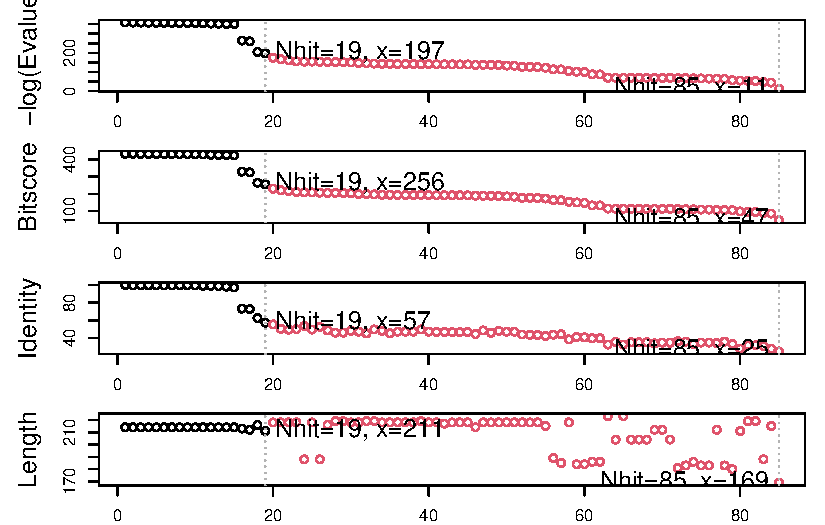
\includegraphics{BIMM143-Lab-9-final_files/figure-pdf/unnamed-chunk-26-1.pdf}

\begin{Shaded}
\begin{Highlighting}[]
\CommentTok{\# y axis is the log of E values because it is difficult to work with extremely small values, often take the log in scenarios like these}
\end{Highlighting}
\end{Shaded}

\begin{Shaded}
\begin{Highlighting}[]
\NormalTok{hits}
\end{Highlighting}
\end{Shaded}

\begin{verbatim}
$hits
   pdb.id   acc      group
1  "1AKE_A" "1AKE_A" "1"  
2  "8BQF_A" "8BQF_A" "1"  
3  "4X8M_A" "4X8M_A" "1"  
4  "6S36_A" "6S36_A" "1"  
5  "8Q2B_A" "8Q2B_A" "1"  
6  "8RJ9_A" "8RJ9_A" "1"  
7  "6RZE_A" "6RZE_A" "1"  
8  "4X8H_A" "4X8H_A" "1"  
9  "3HPR_A" "3HPR_A" "1"  
10 "1E4V_A" "1E4V_A" "1"  
11 "5EJE_A" "5EJE_A" "1"  
12 "1E4Y_A" "1E4Y_A" "1"  
13 "3X2S_A" "3X2S_A" "1"  
14 "6HAP_A" "6HAP_A" "1"  
15 "6HAM_A" "6HAM_A" "1"  
16 "4K46_A" "4K46_A" "1"  
17 "4NP6_A" "4NP6_A" "1"  
18 "3GMT_A" "3GMT_A" "1"  
19 "4PZL_A" "4PZL_A" "1"  

$pdb.id
 [1] "1AKE_A" "8BQF_A" "4X8M_A" "6S36_A" "8Q2B_A" "8RJ9_A" "6RZE_A" "4X8H_A"
 [9] "3HPR_A" "1E4V_A" "5EJE_A" "1E4Y_A" "3X2S_A" "6HAP_A" "6HAM_A" "4K46_A"
[17] "4NP6_A" "3GMT_A" "4PZL_A"

$acc
 [1] "1AKE_A" "8BQF_A" "4X8M_A" "6S36_A" "8Q2B_A" "8RJ9_A" "6RZE_A" "4X8H_A"
 [9] "3HPR_A" "1E4V_A" "5EJE_A" "1E4Y_A" "3X2S_A" "6HAP_A" "6HAM_A" "4K46_A"
[17] "4NP6_A" "3GMT_A" "4PZL_A"

$inds
 [1]  TRUE  TRUE  TRUE  TRUE  TRUE  TRUE  TRUE  TRUE  TRUE  TRUE  TRUE  TRUE
[13]  TRUE  TRUE  TRUE  TRUE  TRUE  TRUE  TRUE FALSE FALSE FALSE FALSE FALSE
[25] FALSE FALSE FALSE FALSE FALSE FALSE FALSE FALSE FALSE FALSE FALSE FALSE
[37] FALSE FALSE FALSE FALSE FALSE FALSE FALSE FALSE FALSE FALSE FALSE FALSE
[49] FALSE FALSE FALSE FALSE FALSE FALSE FALSE FALSE FALSE FALSE FALSE FALSE
[61] FALSE FALSE FALSE FALSE FALSE FALSE FALSE FALSE FALSE FALSE FALSE FALSE
[73] FALSE FALSE FALSE FALSE FALSE FALSE FALSE FALSE FALSE FALSE FALSE FALSE
[85] FALSE

attr(,"class")
[1] "blast"
\end{verbatim}

\begin{Shaded}
\begin{Highlighting}[]
\NormalTok{hits}\SpecialCharTok{$}\NormalTok{pdb.id}
\end{Highlighting}
\end{Shaded}

\begin{verbatim}
 [1] "1AKE_A" "8BQF_A" "4X8M_A" "6S36_A" "8Q2B_A" "8RJ9_A" "6RZE_A" "4X8H_A"
 [9] "3HPR_A" "1E4V_A" "5EJE_A" "1E4Y_A" "3X2S_A" "6HAP_A" "6HAM_A" "4K46_A"
[17] "4NP6_A" "3GMT_A" "4PZL_A"
\end{verbatim}

\begin{Shaded}
\begin{Highlighting}[]
\NormalTok{b}\SpecialCharTok{$}\NormalTok{hit.table}
\end{Highlighting}
\end{Shaded}

\begin{verbatim}
NULL
\end{verbatim}

\begin{Shaded}
\begin{Highlighting}[]
\NormalTok{s }\OtherTok{\textless{}{-}} \ConstantTok{NULL}
\NormalTok{hits}\SpecialCharTok{$}\NormalTok{pdb.id }\OtherTok{\textless{}{-}} \FunctionTok{c}\NormalTok{(}\StringTok{\textquotesingle{}1AKE\_A\textquotesingle{}}\NormalTok{,}\StringTok{\textquotesingle{}6S36\_A\textquotesingle{}}\NormalTok{,}\StringTok{\textquotesingle{}6RZE\_A\textquotesingle{}}\NormalTok{,}\StringTok{\textquotesingle{}3HPR\_A\textquotesingle{}}\NormalTok{,}\StringTok{\textquotesingle{}1E4V\_A\textquotesingle{}}\NormalTok{,}\StringTok{\textquotesingle{}5EJE\_A\textquotesingle{}}\NormalTok{,}\StringTok{\textquotesingle{}1E4Y\_A\textquotesingle{}}\NormalTok{,}\StringTok{\textquotesingle{}3X2S\_A\textquotesingle{}}\NormalTok{,}\StringTok{\textquotesingle{}6HAP\_A\textquotesingle{}}\NormalTok{,}\StringTok{\textquotesingle{}6HAM\_A\textquotesingle{}}\NormalTok{,}\StringTok{\textquotesingle{}4K46\_A\textquotesingle{}}\NormalTok{,}\StringTok{\textquotesingle{}3GMT\_A\textquotesingle{}}\NormalTok{,}\StringTok{\textquotesingle{}4PZL\_A\textquotesingle{}}\NormalTok{)}
\end{Highlighting}
\end{Shaded}

\begin{Shaded}
\begin{Highlighting}[]
\CommentTok{\# Download related PDB files}
\NormalTok{files }\OtherTok{\textless{}{-}} \FunctionTok{get.pdb}\NormalTok{(hits}\SpecialCharTok{$}\NormalTok{pdb.id, }\AttributeTok{path=}\StringTok{"pdbs"}\NormalTok{, }\AttributeTok{split=}\ConstantTok{TRUE}\NormalTok{, }\AttributeTok{gzip=}\ConstantTok{TRUE}\NormalTok{)}
\end{Highlighting}
\end{Shaded}

\begin{verbatim}
Warning in get.pdb(hits$pdb.id, path = "pdbs", split = TRUE, gzip = TRUE):
pdbs/1AKE.pdb.gz exists. Skipping download
\end{verbatim}

\begin{verbatim}
Warning in get.pdb(hits$pdb.id, path = "pdbs", split = TRUE, gzip = TRUE):
pdbs/6S36.pdb.gz exists. Skipping download
\end{verbatim}

\begin{verbatim}
Warning in get.pdb(hits$pdb.id, path = "pdbs", split = TRUE, gzip = TRUE):
pdbs/6RZE.pdb.gz exists. Skipping download
\end{verbatim}

\begin{verbatim}
Warning in get.pdb(hits$pdb.id, path = "pdbs", split = TRUE, gzip = TRUE):
pdbs/3HPR.pdb.gz exists. Skipping download
\end{verbatim}

\begin{verbatim}
Warning in get.pdb(hits$pdb.id, path = "pdbs", split = TRUE, gzip = TRUE):
pdbs/1E4V.pdb.gz exists. Skipping download
\end{verbatim}

\begin{verbatim}
Warning in get.pdb(hits$pdb.id, path = "pdbs", split = TRUE, gzip = TRUE):
pdbs/5EJE.pdb.gz exists. Skipping download
\end{verbatim}

\begin{verbatim}
Warning in get.pdb(hits$pdb.id, path = "pdbs", split = TRUE, gzip = TRUE):
pdbs/1E4Y.pdb.gz exists. Skipping download
\end{verbatim}

\begin{verbatim}
Warning in get.pdb(hits$pdb.id, path = "pdbs", split = TRUE, gzip = TRUE):
pdbs/3X2S.pdb.gz exists. Skipping download
\end{verbatim}

\begin{verbatim}
Warning in get.pdb(hits$pdb.id, path = "pdbs", split = TRUE, gzip = TRUE):
pdbs/6HAP.pdb.gz exists. Skipping download
\end{verbatim}

\begin{verbatim}
Warning in get.pdb(hits$pdb.id, path = "pdbs", split = TRUE, gzip = TRUE):
pdbs/6HAM.pdb.gz exists. Skipping download
\end{verbatim}

\begin{verbatim}
Warning in get.pdb(hits$pdb.id, path = "pdbs", split = TRUE, gzip = TRUE):
pdbs/4K46.pdb.gz exists. Skipping download
\end{verbatim}

\begin{verbatim}
Warning in get.pdb(hits$pdb.id, path = "pdbs", split = TRUE, gzip = TRUE):
pdbs/3GMT.pdb.gz exists. Skipping download
\end{verbatim}

\begin{verbatim}
Warning in get.pdb(hits$pdb.id, path = "pdbs", split = TRUE, gzip = TRUE):
pdbs/4PZL.pdb.gz exists. Skipping download
\end{verbatim}

\begin{verbatim}

  |                                                                            
  |                                                                      |   0%
  |                                                                            
  |=====                                                                 |   8%
  |                                                                            
  |===========                                                           |  15%
  |                                                                            
  |================                                                      |  23%
  |                                                                            
  |======================                                                |  31%
  |                                                                            
  |===========================                                           |  38%
  |                                                                            
  |================================                                      |  46%
  |                                                                            
  |======================================                                |  54%
  |                                                                            
  |===========================================                           |  62%
  |                                                                            
  |================================================                      |  69%
  |                                                                            
  |======================================================                |  77%
  |                                                                            
  |===========================================================           |  85%
  |                                                                            
  |=================================================================     |  92%
  |                                                                            
  |======================================================================| 100%
\end{verbatim}

Next we will use the pdbin() function to alism and also optionally fit
(superimpose) the identified PDB structures

\begin{Shaded}
\begin{Highlighting}[]
\CommentTok{\# Align related PDBs}
\NormalTok{pdbs }\OtherTok{\textless{}{-}} \FunctionTok{pdbaln}\NormalTok{(files, }\AttributeTok{fit =} \ConstantTok{TRUE}\NormalTok{, }\AttributeTok{exefile=}\StringTok{"msa"}\NormalTok{)}
\end{Highlighting}
\end{Shaded}

\begin{verbatim}
Reading PDB files:
pdbs/split_chain/1AKE_A.pdb
pdbs/split_chain/6S36_A.pdb
pdbs/split_chain/6RZE_A.pdb
pdbs/split_chain/3HPR_A.pdb
pdbs/split_chain/1E4V_A.pdb
pdbs/split_chain/5EJE_A.pdb
pdbs/split_chain/1E4Y_A.pdb
pdbs/split_chain/3X2S_A.pdb
pdbs/split_chain/6HAP_A.pdb
pdbs/split_chain/6HAM_A.pdb
pdbs/split_chain/4K46_A.pdb
pdbs/split_chain/3GMT_A.pdb
pdbs/split_chain/4PZL_A.pdb
   PDB has ALT records, taking A only, rm.alt=TRUE
.   PDB has ALT records, taking A only, rm.alt=TRUE
.   PDB has ALT records, taking A only, rm.alt=TRUE
.   PDB has ALT records, taking A only, rm.alt=TRUE
..   PDB has ALT records, taking A only, rm.alt=TRUE
....   PDB has ALT records, taking A only, rm.alt=TRUE
.   PDB has ALT records, taking A only, rm.alt=TRUE
...

Extracting sequences

pdb/seq: 1   name: pdbs/split_chain/1AKE_A.pdb 
   PDB has ALT records, taking A only, rm.alt=TRUE
pdb/seq: 2   name: pdbs/split_chain/6S36_A.pdb 
   PDB has ALT records, taking A only, rm.alt=TRUE
pdb/seq: 3   name: pdbs/split_chain/6RZE_A.pdb 
   PDB has ALT records, taking A only, rm.alt=TRUE
pdb/seq: 4   name: pdbs/split_chain/3HPR_A.pdb 
   PDB has ALT records, taking A only, rm.alt=TRUE
pdb/seq: 5   name: pdbs/split_chain/1E4V_A.pdb 
pdb/seq: 6   name: pdbs/split_chain/5EJE_A.pdb 
   PDB has ALT records, taking A only, rm.alt=TRUE
pdb/seq: 7   name: pdbs/split_chain/1E4Y_A.pdb 
pdb/seq: 8   name: pdbs/split_chain/3X2S_A.pdb 
pdb/seq: 9   name: pdbs/split_chain/6HAP_A.pdb 
pdb/seq: 10   name: pdbs/split_chain/6HAM_A.pdb 
   PDB has ALT records, taking A only, rm.alt=TRUE
pdb/seq: 11   name: pdbs/split_chain/4K46_A.pdb 
   PDB has ALT records, taking A only, rm.alt=TRUE
pdb/seq: 12   name: pdbs/split_chain/3GMT_A.pdb 
pdb/seq: 13   name: pdbs/split_chain/4PZL_A.pdb 
\end{verbatim}

\begin{Shaded}
\begin{Highlighting}[]
\NormalTok{pdbs}
\end{Highlighting}
\end{Shaded}

\begin{verbatim}
                                1        .         .         .         40 
[Truncated_Name:1]1AKE_A.pdb    ----------MRIILLGAPGAGKGTQAQFIMEKYGIPQIS
[Truncated_Name:2]6S36_A.pdb    ----------MRIILLGAPGAGKGTQAQFIMEKYGIPQIS
[Truncated_Name:3]6RZE_A.pdb    ----------MRIILLGAPGAGKGTQAQFIMEKYGIPQIS
[Truncated_Name:4]3HPR_A.pdb    ----------MRIILLGAPGAGKGTQAQFIMEKYGIPQIS
[Truncated_Name:5]1E4V_A.pdb    ----------MRIILLGAPVAGKGTQAQFIMEKYGIPQIS
[Truncated_Name:6]5EJE_A.pdb    ----------MRIILLGAPGAGKGTQAQFIMEKYGIPQIS
[Truncated_Name:7]1E4Y_A.pdb    ----------MRIILLGALVAGKGTQAQFIMEKYGIPQIS
[Truncated_Name:8]3X2S_A.pdb    ----------MRIILLGAPGAGKGTQAQFIMEKYGIPQIS
[Truncated_Name:9]6HAP_A.pdb    ----------MRIILLGAPGAGKGTQAQFIMEKYGIPQIS
[Truncated_Name:10]6HAM_A.pdb   ----------MRIILLGAPGAGKGTQAQFIMEKYGIPQIS
[Truncated_Name:11]4K46_A.pdb   ----------MRIILLGAPGAGKGTQAQFIMAKFGIPQIS
[Truncated_Name:12]3GMT_A.pdb   ----------MRLILLGAPGAGKGTQANFIKEKFGIPQIS
[Truncated_Name:13]4PZL_A.pdb   TENLYFQSNAMRIILLGAPGAGKGTQAKIIEQKYNIAHIS
                                          **^*****  *******  *  *^ *  ** 
                                1        .         .         .         40 

                               41        .         .         .         80 
[Truncated_Name:1]1AKE_A.pdb    TGDMLRAAVKSGSELGKQAKDIMDAGKLVTDELVIALVKE
[Truncated_Name:2]6S36_A.pdb    TGDMLRAAVKSGSELGKQAKDIMDAGKLVTDELVIALVKE
[Truncated_Name:3]6RZE_A.pdb    TGDMLRAAVKSGSELGKQAKDIMDAGKLVTDELVIALVKE
[Truncated_Name:4]3HPR_A.pdb    TGDMLRAAVKSGSELGKQAKDIMDAGKLVTDELVIALVKE
[Truncated_Name:5]1E4V_A.pdb    TGDMLRAAVKSGSELGKQAKDIMDAGKLVTDELVIALVKE
[Truncated_Name:6]5EJE_A.pdb    TGDMLRAAVKSGSELGKQAKDIMDACKLVTDELVIALVKE
[Truncated_Name:7]1E4Y_A.pdb    TGDMLRAAVKSGSELGKQAKDIMDAGKLVTDELVIALVKE
[Truncated_Name:8]3X2S_A.pdb    TGDMLRAAVKSGSELGKQAKDIMDCGKLVTDELVIALVKE
[Truncated_Name:9]6HAP_A.pdb    TGDMLRAAVKSGSELGKQAKDIMDAGKLVTDELVIALVRE
[Truncated_Name:10]6HAM_A.pdb   TGDMLRAAIKSGSELGKQAKDIMDAGKLVTDEIIIALVKE
[Truncated_Name:11]4K46_A.pdb   TGDMLRAAIKAGTELGKQAKSVIDAGQLVSDDIILGLVKE
[Truncated_Name:12]3GMT_A.pdb   TGDMLRAAVKAGTPLGVEAKTYMDEGKLVPDSLIIGLVKE
[Truncated_Name:13]4PZL_A.pdb   TGDMIRETIKSGSALGQELKKVLDAGELVSDEFIIKIVKD
                                ****^*  ^* *^ **   *  ^*   ** *  ^^ ^*^^ 
                               41        .         .         .         80 

                               81        .         .         .         120 
[Truncated_Name:1]1AKE_A.pdb    RIAQEDCRNGFLLDGFPRTIPQADAMKEAGINVDYVLEFD
[Truncated_Name:2]6S36_A.pdb    RIAQEDCRNGFLLDGFPRTIPQADAMKEAGINVDYVLEFD
[Truncated_Name:3]6RZE_A.pdb    RIAQEDCRNGFLLDGFPRTIPQADAMKEAGINVDYVLEFD
[Truncated_Name:4]3HPR_A.pdb    RIAQEDCRNGFLLDGFPRTIPQADAMKEAGINVDYVLEFD
[Truncated_Name:5]1E4V_A.pdb    RIAQEDCRNGFLLDGFPRTIPQADAMKEAGINVDYVLEFD
[Truncated_Name:6]5EJE_A.pdb    RIAQEDCRNGFLLDGFPRTIPQADAMKEAGINVDYVLEFD
[Truncated_Name:7]1E4Y_A.pdb    RIAQEDCRNGFLLDGFPRTIPQADAMKEAGINVDYVLEFD
[Truncated_Name:8]3X2S_A.pdb    RIAQEDSRNGFLLDGFPRTIPQADAMKEAGINVDYVLEFD
[Truncated_Name:9]6HAP_A.pdb    RICQEDSRNGFLLDGFPRTIPQADAMKEAGINVDYVLEFD
[Truncated_Name:10]6HAM_A.pdb   RICQEDSRNGFLLDGFPRTIPQADAMKEAGINVDYVLEFD
[Truncated_Name:11]4K46_A.pdb   RIAQDDCAKGFLLDGFPRTIPQADGLKEVGVVVDYVIEFD
[Truncated_Name:12]3GMT_A.pdb   RLKEADCANGYLFDGFPRTIAQADAMKEAGVAIDYVLEID
[Truncated_Name:13]4PZL_A.pdb   RISKNDCNNGFLLDGVPRTIPQAQELDKLGVNIDYIVEVD
                                *^   *   *^* ** **** **  ^   *^ ^**^^* * 
                               81        .         .         .         120 

                              121        .         .         .         160 
[Truncated_Name:1]1AKE_A.pdb    VPDELIVDRIVGRRVHAPSGRVYHVKFNPPKVEGKDDVTG
[Truncated_Name:2]6S36_A.pdb    VPDELIVDKIVGRRVHAPSGRVYHVKFNPPKVEGKDDVTG
[Truncated_Name:3]6RZE_A.pdb    VPDELIVDAIVGRRVHAPSGRVYHVKFNPPKVEGKDDVTG
[Truncated_Name:4]3HPR_A.pdb    VPDELIVDRIVGRRVHAPSGRVYHVKFNPPKVEGKDDGTG
[Truncated_Name:5]1E4V_A.pdb    VPDELIVDRIVGRRVHAPSGRVYHVKFNPPKVEGKDDVTG
[Truncated_Name:6]5EJE_A.pdb    VPDELIVDRIVGRRVHAPSGRVYHVKFNPPKVEGKDDVTG
[Truncated_Name:7]1E4Y_A.pdb    VPDELIVDRIVGRRVHAPSGRVYHVKFNPPKVEGKDDVTG
[Truncated_Name:8]3X2S_A.pdb    VPDELIVDRIVGRRVHAPSGRVYHVKFNPPKVEGKDDVTG
[Truncated_Name:9]6HAP_A.pdb    VPDELIVDRIVGRRVHAPSGRVYHVKFNPPKVEGKDDVTG
[Truncated_Name:10]6HAM_A.pdb   VPDELIVDRIVGRRVHAPSGRVYHVKFNPPKVEGKDDVTG
[Truncated_Name:11]4K46_A.pdb   VADSVIVERMAGRRAHLASGRTYHNVYNPPKVEGKDDVTG
[Truncated_Name:12]3GMT_A.pdb   VPFSEIIERMSGRRTHPASGRTYHVKFNPPKVEGKDDVTG
[Truncated_Name:13]4PZL_A.pdb   VADNLLIERITGRRIHPASGRTYHTKFNPPKVADKDDVTG
                                *    ^^^ ^ *** *  *** **  ^*****  *** ** 
                              121        .         .         .         160 

                              161        .         .         .         200 
[Truncated_Name:1]1AKE_A.pdb    EELTTRKDDQEETVRKRLVEYHQMTAPLIGYYSKEAEAGN
[Truncated_Name:2]6S36_A.pdb    EELTTRKDDQEETVRKRLVEYHQMTAPLIGYYSKEAEAGN
[Truncated_Name:3]6RZE_A.pdb    EELTTRKDDQEETVRKRLVEYHQMTAPLIGYYSKEAEAGN
[Truncated_Name:4]3HPR_A.pdb    EELTTRKDDQEETVRKRLVEYHQMTAPLIGYYSKEAEAGN
[Truncated_Name:5]1E4V_A.pdb    EELTTRKDDQEETVRKRLVEYHQMTAPLIGYYSKEAEAGN
[Truncated_Name:6]5EJE_A.pdb    EELTTRKDDQEECVRKRLVEYHQMTAPLIGYYSKEAEAGN
[Truncated_Name:7]1E4Y_A.pdb    EELTTRKDDQEETVRKRLVEYHQMTAPLIGYYSKEAEAGN
[Truncated_Name:8]3X2S_A.pdb    EELTTRKDDQEETVRKRLCEYHQMTAPLIGYYSKEAEAGN
[Truncated_Name:9]6HAP_A.pdb    EELTTRKDDQEETVRKRLVEYHQMTAPLIGYYSKEAEAGN
[Truncated_Name:10]6HAM_A.pdb   EELTTRKDDQEETVRKRLVEYHQMTAPLIGYYSKEAEAGN
[Truncated_Name:11]4K46_A.pdb   EDLVIREDDKEETVLARLGVYHNQTAPLIAYYGKEAEAGN
[Truncated_Name:12]3GMT_A.pdb   EPLVQRDDDKEETVKKRLDVYEAQTKPLITYYGDWARRGA
[Truncated_Name:13]4PZL_A.pdb   EPLITRTDDNEDTVKQRLSVYHAQTAKLIDFYRNFSSTNT
                                * *  * ** *^ *  **  *   *  ** ^*         
                              161        .         .         .         200 

                              201        .         .      227 
[Truncated_Name:1]1AKE_A.pdb    T--KYAKVDGTKPVAEVRADLEKILG-
[Truncated_Name:2]6S36_A.pdb    T--KYAKVDGTKPVAEVRADLEKILG-
[Truncated_Name:3]6RZE_A.pdb    T--KYAKVDGTKPVAEVRADLEKILG-
[Truncated_Name:4]3HPR_A.pdb    T--KYAKVDGTKPVAEVRADLEKILG-
[Truncated_Name:5]1E4V_A.pdb    T--KYAKVDGTKPVAEVRADLEKILG-
[Truncated_Name:6]5EJE_A.pdb    T--KYAKVDGTKPVAEVRADLEKILG-
[Truncated_Name:7]1E4Y_A.pdb    T--KYAKVDGTKPVAEVRADLEKILG-
[Truncated_Name:8]3X2S_A.pdb    T--KYAKVDGTKPVAEVRADLEKILG-
[Truncated_Name:9]6HAP_A.pdb    T--KYAKVDGTKPVCEVRADLEKILG-
[Truncated_Name:10]6HAM_A.pdb   T--KYAKVDGTKPVCEVRADLEKILG-
[Truncated_Name:11]4K46_A.pdb   T--QYLKFDGTKAVAEVSAELEKALA-
[Truncated_Name:12]3GMT_A.pdb   E-------NGLKAPA-----YRKISG-
[Truncated_Name:13]4PZL_A.pdb   KIPKYIKINGDQAVEKVSQDIFDQLNK
                                         *                  
                              201        .         .      227 

Call:
  pdbaln(files = files, fit = TRUE, exefile = "msa")

Class:
  pdbs, fasta

Alignment dimensions:
  13 sequence rows; 227 position columns (204 non-gap, 23 gap) 

+ attr: xyz, resno, b, chain, id, ali, resid, sse, call
\end{verbatim}

\subsection{Principal Component
Analysis}\label{principal-component-analysis}

\begin{Shaded}
\begin{Highlighting}[]
\CommentTok{\# Perform PCA}
\NormalTok{pc.xray }\OtherTok{\textless{}{-}} \FunctionTok{pca}\NormalTok{(pdbs)}
\FunctionTok{plot}\NormalTok{(pc.xray)}
\end{Highlighting}
\end{Shaded}

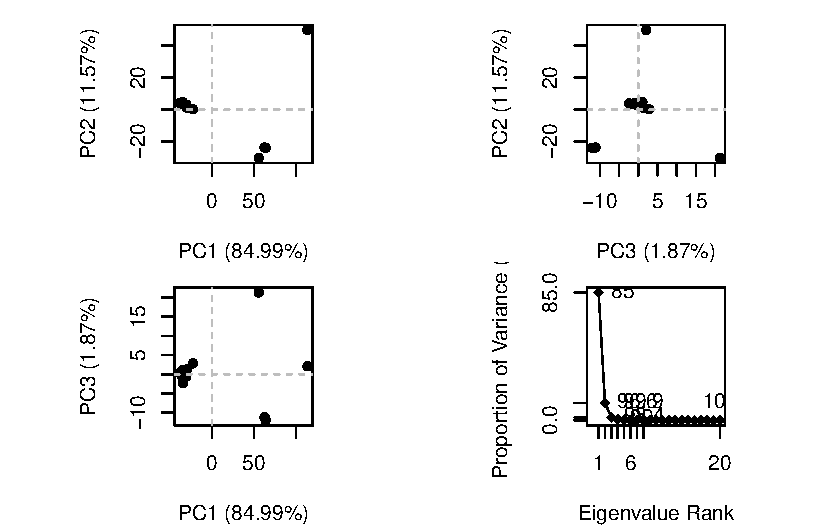
\includegraphics{BIMM143-Lab-9-final_files/figure-pdf/unnamed-chunk-32-1.pdf}

\begin{Shaded}
\begin{Highlighting}[]
\CommentTok{\# Visualize first principal component}
\NormalTok{pc1 }\OtherTok{\textless{}{-}} \FunctionTok{mktrj}\NormalTok{(pc.xray, }\AttributeTok{pc=}\DecValTok{1}\NormalTok{, }\AttributeTok{file=}\StringTok{"pc\_1.pdb"}\NormalTok{)}
\end{Highlighting}
\end{Shaded}

There are many more proteins in the Uniprot website than in our pdb, it
takes years to find the protein structure of all of these proteins

\begin{Shaded}
\begin{Highlighting}[]
\NormalTok{uniprot }\OtherTok{\textless{}{-}} \DecValTok{248838887}
\NormalTok{pdb }\OtherTok{\textless{}{-}} \DecValTok{195610}

\NormalTok{pdb}\SpecialCharTok{/}\NormalTok{uniprot }\SpecialCharTok{*} \DecValTok{100}
\end{Highlighting}
\end{Shaded}

\begin{verbatim}
[1] 0.0786091
\end{verbatim}

\begin{Shaded}
\begin{Highlighting}[]
\CommentTok{\# we only have about 8\% of strcuutres of these proteins }
\end{Highlighting}
\end{Shaded}

Two main approaches to finding structures (both useful but imperfect):

Physics based V(R) = E(bonded) + E(non bonded)

Knowledge based Accuracy is limited by current data availability Not
very clear how to make imporvements




\end{document}
